{\LARGE
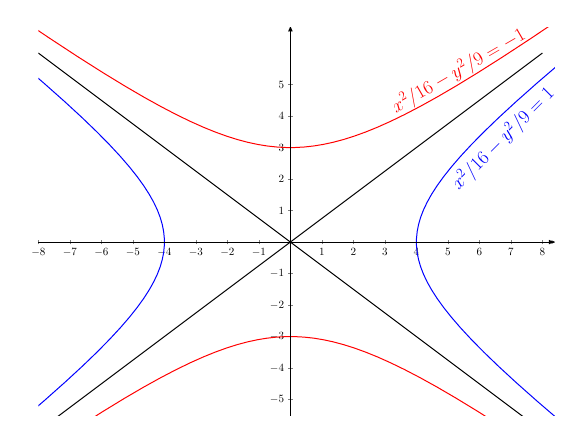
\begin{tikzpicture}[scale=0.4,line width=1pt,>=latex,x=1.0cm,y=1.0cm]
\begin{axis}[x=1.0cm,y=1.0cm,axis lines=middle,%ymajorgrids=true,xmajorgrids=true,
xmin=-8,xmax=8.4,ymin=-5.5,ymax=6.8,
xtick={-8,-7,...,8},
ytick={-5,-4,...,5},]
%\clip(-17.72380254195542,-10.985107966995432) rectangle (20.478992095004248,13.31088776571762);
\draw [samples=50,domain=-0.90:0.90,rotate around={0.:(0.,0.)},xshift=0.cm,yshift=0.cm,line width=0.9pt,color=blue] plot ({4.*(1+(\x)^2)/(1-(\x)^2)},{3.*2*(\x)/(1-(\x)^2)});
\draw [samples=50,domain=-0.9:0.9,rotate around={0.:(0.,0.)},xshift=0.cm,yshift=0.cm,line width=0.9pt,color=blue] plot ({4.*(-1-(\x)^2)/(1-(\x)^2)},{3.*(-2)*(\x)/(1-(\x)^2)});
\draw [samples=50,domain=-0.9:0.9,rotate around={90.:(0.,0.)},xshift=0.cm,yshift=0.cm,line width=0.9pt,color=red] plot ({3.*(1+(\x)^2)/(1-(\x)^2)},{4.*2*(\x)/(1-(\x)^2)});
\draw [samples=50,domain=-0.9:0.9,rotate around={90.:(0.,0.)},xshift=0.cm,yshift=0.cm,line width=0.9pt,color=red] plot ({3.*(-1-(\x)^2)/(1-(\x)^2)},{4.*(-2)*(\x)/(1-(\x)^2)});
\draw [line width=0.9pt] (-8.,-6.)-- (8.,6.);
\draw [line width=0.9pt] (8.,-6.)-- (-8.,6.);
\draw [->,line width=0.9pt] (-8.,0.) -- (8.399903020301497,0.);
\draw [->,line width=0.9pt] (0.,-6.) -- (0.,6.883898551612514);
%\draw [fill=red] (4.083633530431627,5.423006123113449) circle (2.5pt);
\draw[color=red] (5.345122699206521,5.4348306998378435) node {\rotatebox{30}{\LARGE$x^2/16-y^2/9=-1$}};
%\draw [fill=black] (7.425142410045524,3.776465515767476) circle (2.5pt);
\draw[color=blue] (6.753651842404206,3.271468477957376) node {\rotatebox{45}{\LARGE$x^2/16-y^2/9=1$}};
\end{axis}
\end{tikzpicture}}
